\documentclass[usenames,dvipsnames,aspectratio=169]{beamer}
\usepackage{../common/prgBasics}
\usepackage{tabularx}

\title[Lecture 5.]{Programming basics}
\subtitle{(GKNB\_INTA023)}

\begin{document}

%1
\begin{frame}[plain]
  \titlepage
\end{frame}

%2
\begin{frame}{Calculating the surface and volume of a cylinder}
  \begin{columns}[T]
    \column{0.3\linewidth}
      \hfill 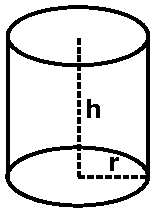
\includegraphics{cylinder.pdf}\\
    \column{0.7\linewidth}
      Tasks:
      \begin{enumerate}
        \item Read the height and radius of the cylinder
        \item Calculate the surface and volume of the cylinder\\
          $V = r^2\pi h$\\
          $S = 2r\pi h + 2r^2\pi = 2r\pi(r+h)$\\
      \end{enumerate}
      \vfill
  \end{columns}
  \begin{center}
    \scalebox{0.85}{
      \begin{tabular}{llll}
      Type & Size & Number representation limits & Precision\\ \hline \noalign{\smallskip}
      float & 4 bytes & $\pm3,4\cdot10^{-38}$ -- $\pm3,4\cdot10^{+38}$ & 6-7 dec. digits\\
      double & 8 bytes & $\pm1,7\cdot10^{-308}$ -- $\pm1,7\cdot10^{+308}$ & 15-16 dec. digits\\
      long double & 10 bytes & $\pm1,2\cdot10^{-4932}$ -- $\pm1,2\cdot10^{+4932}$ & 19 dec. digits
      \end{tabular}
    }
  \end{center}
\end{frame}

%3
\begin{frame}{Calculating the surface and volume of a cylinder}
    \begin{exampleblock}{\textattachfile{cylinder.c}{cylinder.c}}
    \footnotesize
    \lstinputlisting[style=c]{cylinder.c}
  \end{exampleblock}
\end{frame}

%4
\begin{frame}{Calculating the surface and volume of a cylinder}
  Main properties of \kiemel{floating point} literals
  \begin{itemize}
    \item representation limits $\to$ \texttt{float.h}, eg. 
    \begin{description}[\texttt{DBL\_MIN}]
      \item[\texttt{DBL\_MIN}] the least positive normal number representable by type \texttt{double}
      \item[\texttt{DBL\_MAX}] the greatest finite number that can be stored in a \texttt{double}
    \end{description}
    \item the integer or the fractional part of the mantissa may be omitted, but \kiemel{not both} of them!
    \item the decimal point or the exponent (\texttt{e, E}) part may be omitted, but \kiemel{not both} of them!
    \item without any suffix the internal storage type is \texttt{double}
  \end{itemize}
\end{frame}

%5
\begin{frame}{Calculating the surface and volume of a cylinder}
  Main properties of \kiemel{floating point} literals, contd.
  \begin{itemize}
    \item Suffixes to change the internal storage type of a literal:
    \begin{itemize}
      \item \texttt{f}, \texttt{F} (\texttt{float})
      \item \texttt{l}, \texttt{L} (\texttt{long double})
    \end{itemize}
  \end{itemize}
  \begin{exampleblock}{Some floating point literals}
    -5., .3, 5.3, -5e4, 5.67E-12, -1.23e-4l, 5.F
  \end{exampleblock}
  Some of the (not necessarily standardized) literals of \texttt{math.h}
  \begin{itemize}
    \item \texttt{M\_E} -- Euler-constant
    \item \texttt{M\_PI} -- $\pi$
    \item \texttt{M\_SQRT2} -- $\sqrt{2}$
  \end{itemize}
\end{frame}

%6
\begin{frame}[fragile]{Calculating the surface and volume of a cylinder}
  Main properties of \kiemel{integer} literals
  \begin{itemize}
    \item can be given in decimal, octal (\texttt{0}\dots) and hexadecimal (\texttt{0x}\dots, \texttt{0X}\dots) form
    \item suffixes to change the internal storage type:
    \begin{itemize}
      \item \texttt{u}, \texttt{U} (unsigned)
      \item \texttt{l}, \texttt{L} (long)
    \end{itemize}
  \end{itemize}
  \begin{exampleblock}{Integer variables and literals}
    \begin{verbatim}
int i = 1;                unsigned ui = 8u;
int j = 010;  /* == 8 */  long li = 16L;
int k = 0x2A; /* == 42 */ unsigned long uli = 666Ul;
\end{verbatim}
  \end{exampleblock}
\end{frame}

%7
\begin{frame}{Calculating the surface and volume of a cylinder}
  Main properties of \kiemel{integer} literals, contd.
  \begin{itemize}
    \item representation limits of platform-dependent integer types $\to$ \texttt{limits.h}
    \item platform-independent, fixed size integer types, eg. \texttt{int32\_t}, \texttt{uint16\_t} $\rightarrow$ \texttt{stdint.h} (C99).
  \end{itemize}
  \begin{block}{some details of \texttt{limits.h}}
\#  define SCHAR\_MIN     (-128)\\
\#  define UCHAR\_MAX     255\\
\#  define SHRT\_MAX      32767\\
\#  define INT\_MAX       2147483647\\
\#  define ULONG\_MAX     18446744073709551615UL
  \end{block}
\end{frame}

%8
\begin{frame}{Calculating absolute value}
  \begin{columns}[T]
    \column{0.45\linewidth}
      \begin{exampleblock}{\textattachfile{absolute1.c}{absolute1.c}}
        \scriptsize
        \lstinputlisting[style=c]{absolute1.c}
      \end{exampleblock}
    \column{0.45\linewidth}
      \begin{exampleblock}{\textattachfile{absolute2.c}{absolute2.c}}
        \scriptsize
        \lstinputlisting[style=c]{absolute2.c}
      \end{exampleblock}
  \end{columns}
\end{frame}

%9
\begin{frame}{Calculating absolute value}
  Ternary, conditional operator (shorthand for if...else): \kiemel{\texttt{?:}}
  \begin{exampleblock}{if ... else}
    if(\kiemel{logicalExpression}) \{\\
    \hspace{0.5cm} variable = \kiemelZ{valueIfTrue};\\
    \} else \{\\
    \hspace{0.5cm} variable = \kiemelN{valueIfFalse};\\
    \}
  \end{exampleblock}
  \begin{exampleblock}{Ternary operator}
    variable = \kiemel{logicalExpression} ? \kiemelZ{valueIfTrue} : \kiemelN{valueIfFalse};
  \end{exampleblock}
\end{frame}

%10
\begin{frame}{Triangle inequality}
  \begin{exampleblock}{\textattachfile{triangle5.c}{triangle5.c}}
    \tiny
    \vspace{-.3cm}
    \lstinputlisting[style=c]{triangle5.c}
    \vspace{-.3cm}
  \end{exampleblock}
\end{frame}

%11
\begin{frame}{Solving a quadratic equation}
  \begin{exampleblock}{\textattachfile{quadratic.c}{quadratic.c} $x_{1,2} = \frac{-b\pm\sqrt{b^2 - 4ac}}{2a}$}
    \tiny
    \lstinputlisting[style=c]{quadratic.c}
  \end{exampleblock}
\end{frame}

%12
\begin{frame}{Solving a quadratic equation}
  Mathematical functions
  \begin{itemize}
    \item Standard function libraries $\rightarrow$ portability
    \item Header to be included: \texttt{math.h}
    \item GCC: linking of the floating-point library must be explicitely stated, eg.:\\
    \texttt{gcc -Wall -o quadratic quadratic.c -lm }
    \item The type of function parameters and return values are usually \texttt{double}
    \item Argument and return value of trigonometric functions are specified in \kiemel{radians}
  \end{itemize}
\end{frame}

%13
\begin{frame}{Solving a quadratic equation}
  Some often used mathematical function
  \vfill
  \footnotesize
  \begin{tabular}{p{.45\textwidth}p{.45\textwidth}}
    Prototype & Goal\\ \hline
    \texttt{double ceil(double x)} & returns the smallest integral value that is not less than x\\
    \texttt{double cos(double x)} & cosine\\
    \texttt{double cosh(double x)} & hyperbolic cosine\\
    \texttt{double exp(double x)} & base-e exponential function\\
    \texttt{double fabs(double x)} & absolute value of floating-point number\\
    \texttt{double fmod(double x, double~y)} & computes the floating-point remainder of dividing x by y\\
    \texttt{double log(double x)} & natural logarithmic function\\
    \texttt{double log10(double x)} & base-10 logarithmic function\\
    \texttt{double pow(double x, double~y)} & power function\\
    \texttt{double sqrt(double x)} & square root
  \end{tabular}
\end{frame}

%14
\begin{frame}{Fahrenheit -- Celsius conversion}
  $C = \frac{5}{9}(F-32)$
  \begin{columns}[T]
    \column{0.67\linewidth}
      \begin{exampleblock}{\textattachfile{fahrCels1.c}{fahrCels1.c}}
        \scriptsize
        \lstinputlisting[style=c,numbers=left]{fahrCels1.c}
      \end{exampleblock}
    \column{0.33\linewidth}
      \begin{block}{Output}
        \scriptsize
        Fahrenheit --> Celsius\\
        Fahrenheit: 72\\
        Celsius: 0.000000\\
      \end{block}
      Remarks:
      \begin{itemize}
        \item \texttt{5/9} $\to$ always 0!
        \item \texttt{f-32} $\to$ implicit type conversion to \texttt{double}
      \end{itemize}
  \end{columns}
\end{frame}

%15
\begin{frame}{Fahrenheit -- Celsius conversion}
  \kiemel{Implicit/automatic type conversion}: binary operators work with the same type of operands. In general, if types differ the smaller/more inaccurate operand is converted to the bigger/more accurate type.
  \begin{center}
    \[
      \left\downarrow\mbox{
      \begin{tabular}{ll}
        one of the operands & the other operand\\ \hline
        \texttt{long double} & \emph{anything}$\rightarrow$\texttt{long double}\\
        \texttt{double} & \emph{anything}$\rightarrow$\texttt{double}\\
        \texttt{float} & \emph{anything}$\rightarrow$\texttt{float}\\
        \emph{integer promotion} & \emph{integer promotion}\\
        \texttt{unsigned long} & \emph{anything}$\rightarrow$\texttt{unsigned long}\\
        \texttt{long}$\rightarrow$(\texttt{unsigned}) \texttt{long} & \texttt{unsigned int}$\rightarrow$(\texttt{unsigned})
        \texttt{long}\\
        \texttt{long} & \emph{anything}$\rightarrow$\texttt{long}\\
        \texttt{unsigned int} & \emph{anything}$\rightarrow$\texttt{unsigned int}\\
        int & int
      \end{tabular}}
      \right.
    \]
  \end{center}
\end{frame}

%16
\begin{frame}{Fahrenheit -- Celsius conversion}
  \kiemel{Integer promotion}
  \begin{center}
    \small
    \begin{tabular}{lll}
      Original type & Converted type & Conversion method\\ \hline
      \texttt{char} & \texttt{int} & According to the default (signed/unsigned) char type.\\
      \texttt{unsigned char} & \texttt{int} & Extension with zero-valued bits.\\
      \texttt{signed char} & \texttt{int} & Extension with the value of the sign bit.\\
      \texttt{short int} & \texttt{int} & Extension with the value of the sign bit.\\
      \texttt{unsigned short} & \texttt{unsigned int} & Extension with zero-valued bits.\\
    \end{tabular}
  \end{center}
  Attention!
  \begin{itemize}
    \item Conversions need time!
    \item A string is never converted to arithmetic value implicitely!
  \end{itemize}
\end{frame}

%17
\begin{frame}[fragile]{Fahrenheit -- Celsius conversion}
  \kiemel{Explicit type conversion} (Type casting)
  \begin{exampleblock}{\textattachfile{fahrCels3.c}{fahrCels3.c}}
    \lstinputlisting[style=c,firstline=8,lastline=9,firstnumber=8,numbers=left]{fahrCels3.c}
  \end{exampleblock}
  \begin{block}{Output}
    \begin{verbatim}
Fahrenheit --> Celsius
Fahrenheit: 72
Celsius: 22.222222
\end{verbatim}
  \end{block}
\end{frame}

%18
\begin{frame}{Fahrenheit -- Celsius conversion}
  \begin{columns}[T]
    \column{0.45\linewidth}
      \begin{exampleblock}{\textattachfile{fahrCels2.c}{fahrCels2.c}}
        \tiny
        \lstinputlisting[style=c,numbers=left,firstline=8,lastline=9,firstnumber=8]{fahrCels2.c}
      \end{exampleblock}
      \begin{block}{Output}
        \scriptsize
        Celsius: 22.222222\\
      \end{block}
      \begin{exampleblock}{\textattachfile{fahrCels4.c}{fahrCels4.c}}
        \tiny
        \lstinputlisting[style=c,numbers=left,firstline=8,lastline=9,firstnumber=8]{fahrCels4.c}
      \end{exampleblock}
      \begin{block}{Output}
        \scriptsize
        Celsius: 22.222222\\
      \end{block}
    \column{0.51\linewidth}
      \begin{exampleblock}{\textattachfile{fahrCels3.c}{fahrCels3.c}}
        \tiny
        \lstinputlisting[style=c,numbers=right,firstline=8,lastline=9,firstnumber=8]{fahrCels3.c}
      \end{exampleblock}
      \begin{block}{Output}
        \scriptsize
        Celsius: 22.222222\\
      \end{block}
      \begin{exampleblock}{\textattachfile{fahrCels5.c}{fahrCels5.c}}
        \tiny
        \lstinputlisting[style=c,numbers=right,firstline=8,lastline=9,firstnumber=8]{fahrCels5.c}
      \end{exampleblock}
      \begin{block}{Output}
        \scriptsize
        Celsius: 0.000000\\
      \end{block}
  \end{columns}
\end{frame}

%19
\begin{frame}{Precedence and associativity of operators}
  \begin{center}
    \scriptsize
    \begin{tabular}{ll}
    Operator & Associativity \\ \hline\hline
    a++ a$--$ & \multirow{2}{*}{left to right} \\ 
    \kiemel{fn() array[]} & \\ \hline
    ++a $--$a & \multirow{7}{*}{right to left} \\
    +a $-$a & \\
    ! & \\
    \kiemel{(type)} & \\
    \kiemel{*pointer} & \\
    \kiemel{\&variable} & \\
    sizeof & \\ \hline
    a*b a/b a\%b & \multirow{6}{*}{left to right} \\
    a+b a$-$b & \\
    < <= > >= & \\
    == != & \\
    \&\& & \\
    || & \\ \hline
    \kiemel{a?b:c} & \multirow{2}{*}{right to left}\\
    = += $-$= *= /= \%= & \\ \hline
    , & left to right \\ \hline
    \end{tabular}
  \end{center}
\end{frame}

%20
\begin{frame}{\texttt{for} loop}
  \scriptsize
  \texttt{for(}<\emph{init-expression}>\texttt{;} <\emph{repeat-expression}>\texttt{;} <\emph{increment-expression}>\texttt{)} 
\emph{statement}
  \begin{enumerate}
    \item evaluating \emph{init-expression} if it is provided
    \item executing \emph{statement}, if the value of \emph{repeat-expression} is true
    \item evaluating \emph{increment-expression} if it is provided, then go to 2
  \end{enumerate}
  All \emph{expressions} can be empty or compound using the comma operator. The empty \emph{repeat-expression} evaluates to \texttt{true}.
  Usual scenario:
  \begin{exampleblock}{while}
    \kiemel{loopVariable = initialValue;}\\
    while(\kiemelZ{loopVariable < finalValue}) \{\\
      \hspace{0.5cm} loopBody;\\
      \hspace{0.5cm} \kiemelN{loopVariable += step;}\\
    \}\\
  \end{exampleblock}
  \begin{exampleblock}{for}
    for(\kiemel{loopVariable=initialValue}; \kiemelZ{loopVariable<finalValue}; \kiemelN{loopVariable += step}) \{\\
      \hspace{0.5cm} loopBody;\\
    \}\\
  \end{exampleblock}
\end{frame}

%21
\begin{frame}{\texttt{for} loop}
  Reading N numbers, storing and printing of them in reverse order
  \begin{columns}[T]
    \column{0.4\linewidth}
      \begin{exampleblock}{\textattachfile{reverse1.c}{reverse1.c}}
        \tiny
        \lstinputlisting[style=c,numbers=left,linerange={5-16},firstnumber=5]{reverse1.c}
      \end{exampleblock}
    \column{0.5\linewidth}
      \begin{exampleblock}{\textattachfile{reverse3.c}{reverse3.c}}
        \tiny
        \lstinputlisting[style=c,numbers=right,linerange={5-14},firstnumber=5]{reverse3.c}
      \end{exampleblock}
  \end{columns}
\end{frame}

%22
\begin{frame}{\texttt{for} loop}
  General scenario:
  \vspace{-.3cm}
  \begin{columns}[T]
    \column{0.33\textwidth}
      \begin{exampleblock}{while}
        \kiemel{statement1;}\\
        while(\kiemelZ{condition}) \{\\
          \hspace{0.5cm} statement2;\\
          \hspace{0.5cm} \kiemelN{statement3;}\\
        \}\\
      \end{exampleblock}
    \column{0.67\textwidth}
      \begin{exampleblock}{for}
        for(\kiemel{statement1}; \kiemelZ{condition}; \kiemelN{statement3}) \{\\
          \hspace{0.5cm} statement2;\\
        \}\\
      \end{exampleblock}
  \end{columns}
  \vfill
  Converting a decimal number to binary number system
  \vspace{-.3cm}
  \begin{columns}[T]
    \column{0.5\linewidth}
      \begin{exampleblock}{\textattachfile{dectobin2.c}{dectobin2.c}}
        \tiny
        \lstinputlisting[style=c,firstline=8,lastline=12,numbers=left,firstnumber=8]{dectobin2.c}
      \end{exampleblock}
    \column{0.5\linewidth}
      \begin{exampleblock}{\textattachfile{dectobin3.c}{dectobin3.c}}
        \tiny
        \lstinputlisting[style=c,firstline=8,lastline=12,numbers=right,firstnumber=8]{dectobin3.c}
      \end{exampleblock}
  \end{columns}
\end{frame}

%23
\begin{frame}{\texttt{for} loop}
  Mirroring a word in place
  \begin{columns}[T]
  \column{0.45\linewidth}
    \begin{exampleblock}{\textattachfile{mirror1.c}{mirror1.c}}
      \tiny
      \vspace{-.3cm}
      \lstinputlisting[style=c]{mirror1.c}
      \vspace{-.3cm}
    \end{exampleblock}
  \column{0.45\linewidth}
    \begin{exampleblock}{\textattachfile{mirror2.c}{mirror2.c}}
      \tiny
      \vspace{-.3cm}
      \lstinputlisting[style=c,numbers=right]{mirror2.c}
      \vspace{-.3cm}
    \end{exampleblock}
  \end{columns}
\end{frame}

%24
\begin{frame}[fragile]{\texttt{for} loop}
  \begin{columns}[T]
    \column{0.6\linewidth}
      \begin{exampleblock}{\textattachfile{fahrCels6.c}{fahrCels6.c}}
        \scriptsize
        \vspace{-.3cm}
        \lstinputlisting[style=c]{fahrCels6.c}
        \vspace{-.3cm}
      \end{exampleblock}
    \column{0.4\linewidth}
      \begin{block}{Output}
        \scriptsize
        \begin{verbatim}
Fahrenheit      Celsius
----------      --------
0.000000        -17.777778
10.000000       -12.222222
20.000000       -6.666667
30.000000       -1.111111
40.000000       4.444444
50.000000       10.000000
60.000000       15.555556
70.000000       21.111111
80.000000       26.666667
90.000000       32.222222
100.000000      37.777778
110.000000      43.333333
120.000000      48.888889
130.000000      54.444444
140.000000      60.000000
150.000000      65.555556
\end{verbatim}
      \end{block}
  \end{columns}
\end{frame}

\end{document}
